\documentclass[10pt,a4paper]{article}
\usepackage[a4paper]{geometry}

\usepackage{polski}
\usepackage{xltxtra}
\usepackage{hyperref}
\hypersetup{
    pdftitle={Sprawozdanie z laboratorium nr 2 z przedmiotu Technika cyfrowa},%
    pdfauthor={Tomasz Cudziło, Łukasz Gwiazda, Andrzej Tolarczyk},%
    colorlinks=true,        % false: boxed links; true: colored links
    linkcolor=black,        % color of internal links
    citecolor=green,        % color of links to bibliography
    filecolor=magenta,      % color of file links
    urlcolor=cyan,          % color of external links
    unicode=true,           % non-Latin characters in Acrobat’s bookmarks
    pdfstartview={FitH},    % fits the width of the page to the window
    pdfnewwindow=true       % links in new window
}
\usepackage{booktabs}
\usepackage{multirow}
\usepackage{amsmath}
\usepackage{multicol}
\usepackage{pdfpages}

%% tweak fonts
\defaultfontfeatures{Mapping=tex-text}
\setromanfont{Charis SIL}
\setsansfont[Scale=MatchLowercase]{Helvetica Neue}
\setmonofont[Scale=MatchLowercase]{Menlo}
\linespread{1.25}

\newcommand{\f}[1]{\texttt{#1}}
\newcommand{\ol}[1]{\overline{#1}}



\begin{document}

\title{
  \textsc{Politechnika Warszawska}\\
  \textsc{Wydział Elektryczny}\\[18pt]
  Sprawozdanie z~laboratorium nr~2\\z~przedmiotu \emph{Technika cyfrowa}
}
\date{}
\maketitle

\begin{tabular*}{\textwidth}{@{\extracolsep{\fill}}llll}
  \toprule
  % \multicolumn{4}{c}{\Large\bf Politechnika Warszawska} \\
  % \addlinespace
  % \multicolumn{4}{c}{\Large\bf Wydział Elektryczny} \\
  % \midrule
  % \multicolumn{4}{c}{\large\bf Układy techniki cyfrowej --- laboratorium} \\
  % \midrule
  \multicolumn{1}{l}{\bf Imię i nazwisko: } & \multicolumn{1}{l}{\bf Data zajęć: } & \multicolumn{2}{l}{ \bf Ocena: } \\
  \multicolumn{1}{l}{Tomasz Cudziło} & \multicolumn{1}{l}{12 marca 2012} & & \\
  \multicolumn{1}{l}{Łukasz Gwiazda} & & & \\
  \multicolumn{1}{l}{Andrzej Tolarczyk} & & & \\
  \midrule
  \multicolumn{1}{l}{\bf{Rok akademicki: }} & \bf{Kierunek: } & \bf{Nr grupy: } & \bf{Nr zespołu: } \\
  \multicolumn{1}{l}{2011/2012} & Informatyka & 2 & 3 \\
  \midrule
  \multicolumn{4}{l}{\bf{Ćwiczenie: }} \\
  \multicolumn{4}{l}{} \\
  \bottomrule
\end{tabular*}
\pagebreak


\section*{Tablica prawdy układu}
\begin{table}[!ht]
  \centering
  \begin{tabular}{r|cccc|ccccccc}
            & \multicolumn{4}{c|}{Wejścia} & \multicolumn{7}{c}{Wyjścia} \\
            & \f{a} & \f{b} & \f{c} & \f{d} & \f{a} & \f{b} & \f{c} & \f{d} & \f{e} & \f{f} & \f{g} \\
    \midrule
    \f{ 1.} & \f{0} & \f{0} & \f{0} & \f{0} & \f{1} & \f{1} & \f{1} & \f{0} & \f{0} & \f{0} & \f{1} \\
    \f{ 2.} & \f{0} & \f{0} & \f{0} & \f{1} & \f{0} & \f{0} & \f{0} & \f{1} & \f{1} & \f{1} & \f{1} \\
    \f{ 3.} & \f{0} & \f{0} & \f{1} & \f{0} & \f{0} & \f{0} & \f{0} & \f{1} & \f{0} & \f{0} & \f{0} \\
    \f{ 4.} & \f{0} & \f{0} & \f{1} & \f{1} & \f{1} & \f{1} & \f{0} & \f{0} & \f{0} & \f{1} & \f{0} \\
    \f{ 5.} & \f{0} & \f{1} & \f{0} & \f{0} & \f{0} & \f{0} & \f{1} & \f{0} & \f{0} & \f{1} & \f{1} \\
    \f{ 6.} & \f{0} & \f{1} & \f{0} & \f{1} & \f{0} & \f{0} & \f{0} & \f{0} & \f{0} & \f{1} & \f{1} \\
    \f{ 7.} & \f{0} & \f{1} & \f{1} & \f{0} & \f{0} & \f{0} & \f{0} & \f{1} & \f{0} & \f{0} & \f{1} \\
    \f{ 8.} & \f{0} & \f{1} & \f{1} & \f{1} & \f{0} & \f{0} & \f{1} & \f{0} & \f{0} & \f{0} & \f{1} \\
    \f{ 9.} & \f{1} & \f{0} & \f{0} & \f{0} & \f{0} & \f{0} & \f{0} & \f{0} & \f{0} & \f{0} & \f{1} \\
    \f{10.} & \f{1} & \f{0} & \f{0} & \f{1} & \f{0} & \f{0} & \f{0} & \f{0} & \f{1} & \f{1} & \f{0} \\
    \f{11.} & \f{1} & \f{0} & \f{1} & \f{0} & \f{-} & \f{-} & \f{-} & \f{-} & \f{-} & \f{-} & \f{-} \\
    \f{12.} & \f{1} & \f{0} & \f{1} & \f{1} & \f{-} & \f{-} & \f{-} & \f{-} & \f{-} & \f{-} & \f{-} \\
    \f{13.} & \f{1} & \f{1} & \f{0} & \f{0} & \f{-} & \f{-} & \f{-} & \f{-} & \f{-} & \f{-} & \f{-} \\
    \f{14.} & \f{1} & \f{1} & \f{0} & \f{1} & \f{-} & \f{-} & \f{-} & \f{-} & \f{-} & \f{-} & \f{-} \\
    \f{15.} & \f{1} & \f{1} & \f{1} & \f{0} & \f{-} & \f{-} & \f{-} & \f{-} & \f{-} & \f{-} & \f{-} \\
    \f{16.} & \f{1} & \f{1} & \f{1} & \f{1} & \f{-} & \f{-} & \f{-} & \f{-} & \f{-} & \f{-} & \f{-} \\
  \end{tabular}
\end{table}
\pagebreak



\section*{Tablice prawdy poszczególnych segmentów}

\begin{table}[!ht]
  \centering
  \begin{minipage}{0.3\linewidth}
    \centering
    \begin{tabular}{c|cccc}
             & \f{00} & \f{01} & \f{11} & \f{10} \\
      \midrule
      \f{00} &  \f{1} &  \f{0} &  \f{1} &  \f{0} \\
      \f{01} &  \f{0} &  \f{0} &  \f{0} &  \f{0} \\
      \f{11} &  \f{-} &  \f{-} &  \f{-} &  \f{-} \\
      \f{10} &  \f{0} &  \f{0} &  \f{-} &  \f{-} \\
    \end{tabular}
    \caption{Segment \f{a}.}
  \end{minipage}
  \quad
  \begin{minipage}{0.3\linewidth}
    \centering
    \begin{tabular}{c|cccc}
             & \f{00} & \f{01} & \f{11} & \f{10} \\
      \midrule
      \f{00} &  \f{1} &  \f{0} &  \f{1} &  \f{0} \\
      \f{01} &  \f{0} &  \f{0} &  \f{0} &  \f{0} \\
      \f{11} &  \f{-} &  \f{-} &  \f{-} &  \f{-} \\
      \f{10} &  \f{0} &  \f{0} &  \f{-} &  \f{-} \\
    \end{tabular}
    \caption{Segment \f{b}.}
  \end{minipage}
  \quad
  \begin{minipage}{0.3\linewidth}
    \centering
    \begin{tabular}{c|cccc}
             & \f{00} & \f{01} & \f{11} & \f{10} \\
      \midrule
      \f{00} &  \f{1} &  \f{0} &  \f{0} &  \f{0} \\
      \f{01} &  \f{1} &  \f{0} &  \f{1} &  \f{0} \\
      \f{11} &  \f{-} &  \f{-} &  \f{-} &  \f{-} \\
      \f{10} &  \f{0} &  \f{0} &  \f{-} &  \f{-} \\
    \end{tabular}
    \caption{Segment \f{c}.}
  \end{minipage}
\end{table}

\begin{table}[!ht]
  \centering
  \begin{minipage}{0.3\linewidth}
    \centering
    \begin{tabular}{c|cccc}
             & \f{00} & \f{01} & \f{11} & \f{10} \\
      \midrule
      \f{00} &  \f{0} &  \f{1} &  \f{0} &  \f{1} \\
      \f{01} &  \f{0} &  \f{0} &  \f{0} &  \f{1} \\
      \f{11} &  \f{-} &  \f{-} &  \f{-} &  \f{-} \\
      \f{10} &  \f{0} &  \f{0} &  \f{-} &  \f{-} \\
    \end{tabular}
    \caption{Segment \f{d}.}
  \end{minipage}
  \quad
  \begin{minipage}{0.3\linewidth}
    \centering
    \begin{tabular}{c|cccc}
              & \f{00} & \f{01} & \f{11} & \f{10} \\
      \midrule
      \f{00} &  \f{0} &  \f{1} &  \f{0} &  \f{0} \\
      \f{01} &  \f{0} &  \f{0} &  \f{0} &  \f{0} \\
      \f{11} &  \f{-} &  \f{-} &  \f{-} &  \f{-} \\
      \f{10} &  \f{0} &  \f{1} &  \f{-} &  \f{-} \\
    \end{tabular}
    \caption{Segment \f{e}.}
  \end{minipage}
  \quad
  \begin{minipage}{0.3\linewidth}
    \centering
    \begin{tabular}{c|cccc}
             & \f{00} & \f{01} & \f{11} & \f{10} \\
      \midrule
      \f{00} &  \f{0} &  \f{1} &  \f{1} &  \f{0} \\
      \f{01} &  \f{1} &  \f{1} &  \f{0} &  \f{0} \\
      \f{11} &  \f{-} &  \f{-} &  \f{-} &  \f{-} \\
      \f{10} &  \f{0} &  \f{1} &  \f{-} &  \f{-} \\
    \end{tabular}
    \caption{Segment \f{f}.}
  \end{minipage}
\end{table}

\begin{table}[!ht]
  \centering
  \begin{minipage}{0.3\linewidth}
    \centering
    \begin{tabular}{c|cccc}
             & \f{00} & \f{01} & \f{11} & \f{10} \\
      \midrule
      \f{00} &  \f{1} &  \f{1} &  \f{0} &  \f{0} \\
      \f{01} &  \f{1} &  \f{1} &  \f{1} &  \f{1} \\
      \f{11} &  \f{-} &  \f{-} &  \f{-} &  \f{-} \\
      \f{10} &  \f{1} &  \f{0} &  \f{-} &  \f{-} \\
    \end{tabular}
    \caption{Segment \f{g}.}
  \end{minipage}
\end{table}
\pagebreak



\section*{Równania układu po minimalizacji}

\begin{align*}
  f_a(abcd) &= \ol{b} \cdot \ol{a} \cdot (c + \ol{d}) \cdot (\ol{c} + d) \\
            &= \ol{b} \cdot \ol{a} \cdot \ol{\ol{c} \cdot d} \cdot \ol{c \cdot \ol{d}} \\
  & \\
  f_b(abcd) &= f_a(abcd) \\
  & \\
  f_c(abcd) &= \ol{a} \cdot (b + \ol{c}) \cdot (\ol{c} + d) \cdot (c + \ol{d}) \\
            &= \ol{a} \cdot \ol{\ol{b} \cdot c} \cdot \ol{c \cdot \ol{d}} \cdot \ol{\ol{c} \cdot d} \\
  & \\
  f_d(abcd) &= \ol{a} \cdot (c + d) \cdot (\ol{c} + \ol{d}) \cdot (\ol{b} + c) \\
            &= \ol{a} \cdot \ol{\ol{c} \cdot \ol{d}} \cdot \ol{c \cdot d} \cdot \ol{b \cdot \ol{c}} \\
  & \\
  f_e(abcd) &= d \cdot \ol{c} \cdot \ol{b} \\
  & \\
  f_f(abcd) &= (b + d) \cdot (\ol{b} + \ol{c}) \\
            &= \ol{\ol{b} \cdot \ol{d}} \cdot \ol{b \cdot c} \\
  & \\
  f_g(abcd) &= (\ol{a} + \ol{d}) \cdot (b + \ol{c}) \\
            &= \ol{a \cdot d} \cdot \ol{\ol{b} \cdot c} \\
\end{align*}



\section*{Równania unikalnych układów}

\begin{multicols}{3}
  \begin{enumerate}
    \item $\ol{\ol{c} \cdot d}$
    \item $\ol{c \cdot \ol{d}}$
    \item $\ol{\ol{b} \cdot c}$
    \item $\ol{\ol{c} \cdot \ol{d}}$
    \item $\ol{c \cdot d}$
    \item $\ol{b \cdot \ol{c}}$
    \item $\ol{\ol{b} \cdot \ol{d}}$
    \item $\ol{b \cdot c}$
    \item $\ol{a \cdot d}$
  \end{enumerate}
\end{multicols}



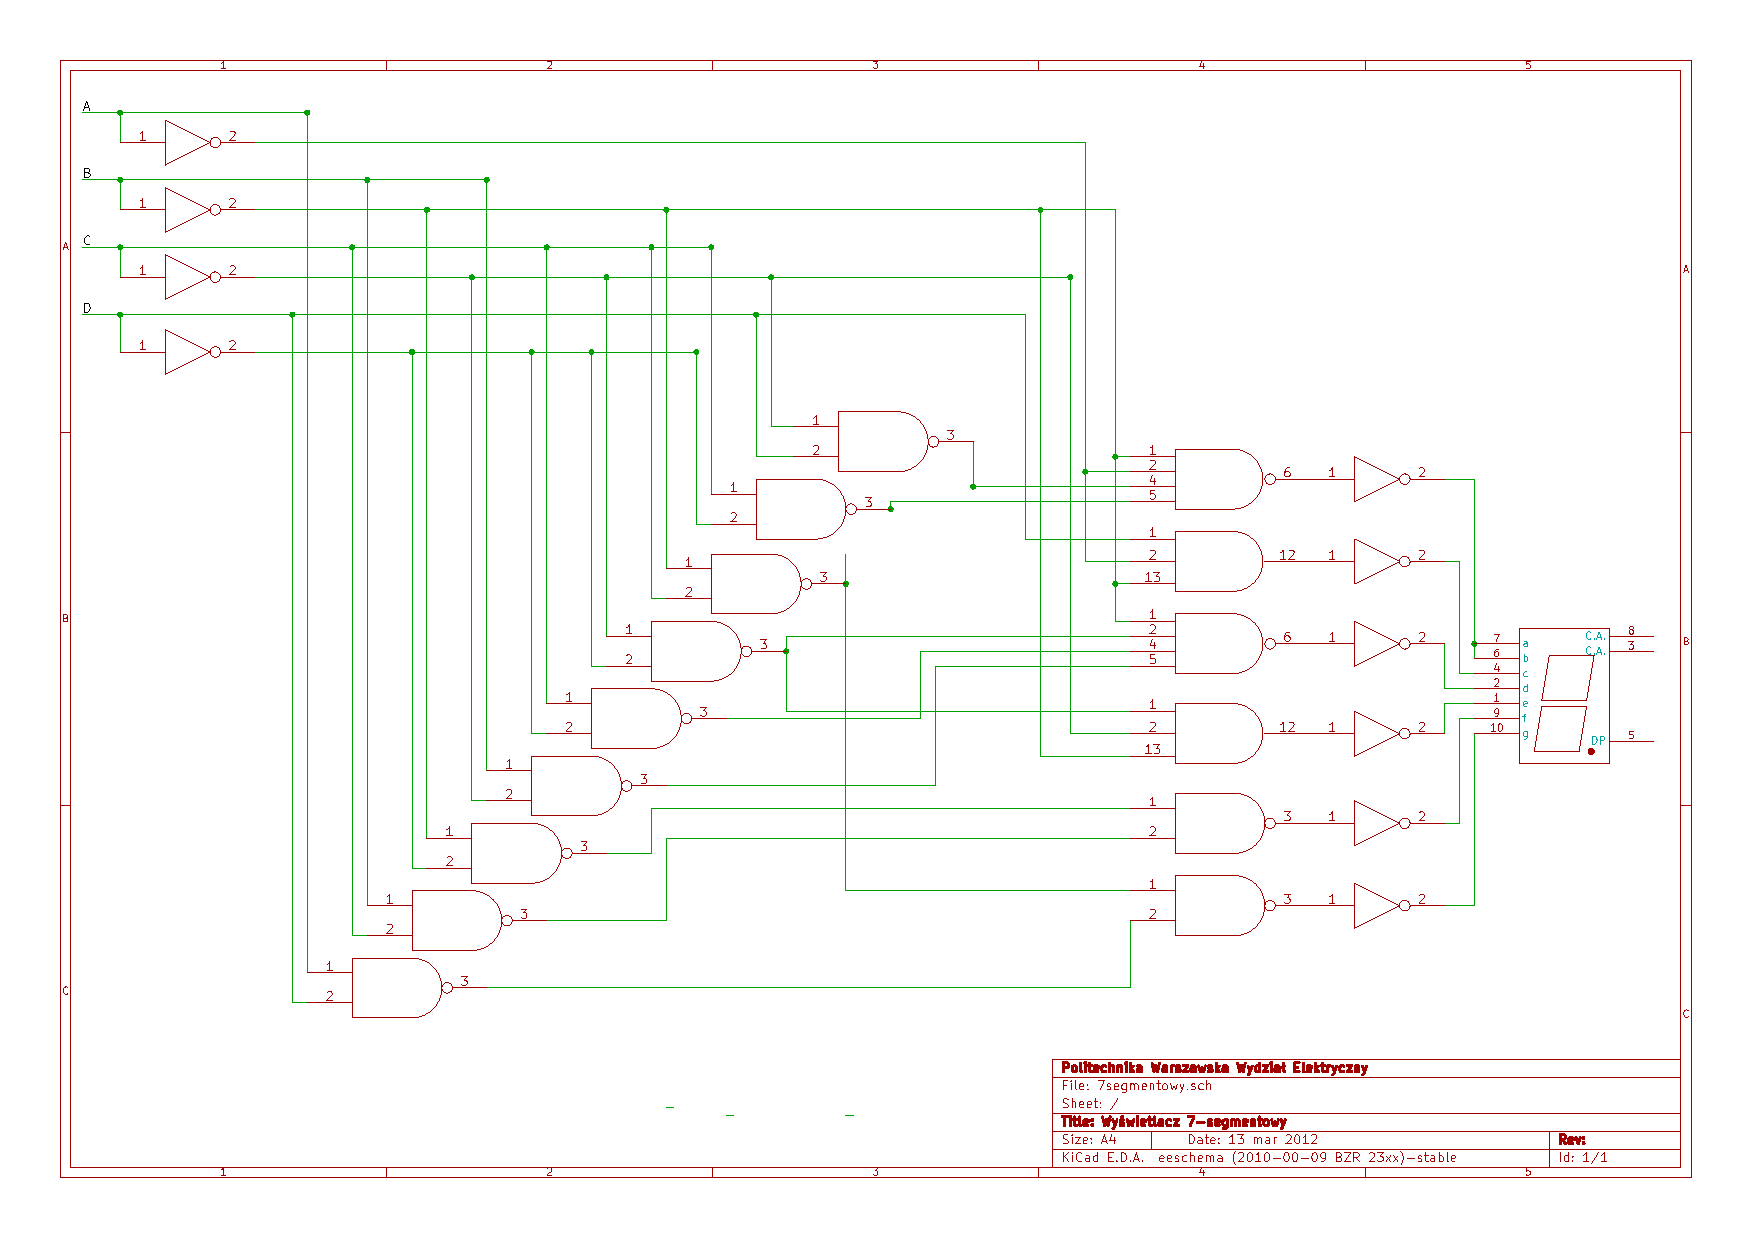
\includepdf[landscape]{figury/schemat-bramek}



\end{document}
